\documentclass[11pt]{article}

\usepackage[a4paper,bindingoffset=0.2in,%
            left=.75in,right=.75in,top=1in,bottom=1in,%
            footskip=.25in]{geometry}

\usepackage[utf8]{inputenc} % Required for inputting international characters
\usepackage[T1]{fontenc} % Output font encoding for international characters

\usepackage{times}
\usepackage{indentfirst}
\usepackage{graphicx}
\usepackage{hyperref}

\setlength{\parskip}{1em}


\begin{document}

%----------------------------------------------------------------------------------------
%	TITLE PAGE
%----------------------------------------------------------------------------------------

\begin{titlepage} % Suppresses displaying the page number on the title page and the subsequent page counts as page 1
	\newcommand{\HRule}{\rule{\linewidth}{0.5mm}} % Defines a new command for horizontal lines, change thickness here
	
	\center % Centre everything on the page
	
	%------------------------------------------------
	%	Headings
	%------------------------------------------------
	
	\textsc{\LARGE Carleton University}\\[1.5cm] 
	
	
	%------------------------------------------------
	%	Title
	%------------------------------------------------
	
	\HRule\\[0.4cm]
	
	{\huge\bfseries Asynchronous Graph Programming Compiler Proposal}\\[0.4cm] 
	
	\HRule\\[1.5cm]
	
	%------------------------------------------------
	%	Author(s)
	%------------------------------------------------
	
	\begin{minipage}{0.4\textwidth}
		\begin{flushleft}
			\large
			\textit{Authors}\\
			Andrew Foster \textsc{101041196}\\
			Nicholas Porter \textsc{101079185}\\
			Sean Wallach \textsc{101035088} 
		\end{flushleft}
	\end{minipage}
	~
	\begin{minipage}{0.4\textwidth}
		\begin{flushright}
			\large
			\textit{Supervisor}\\
			Prof. Garcia 
		\end{flushright}
	\end{minipage}
	
	
	
	%------------------------------------------------
	%	Date
	%------------------------------------------------
	
	\vfill\vfill\vfill % Position the date 3/4 down the remaining page
	
	{\large
	November 2, 2020} 
	
	%------------------------------------------------
	%	Logo
	%------------------------------------------------
	
	%\vfill\vfill
	%\includegraphics[width=0.2\textwidth]{placeholder.jpg}\\[1cm] % Include a department/university logo - this will require the graphicx package
	 
	%----------------------------------------------------------------------------------------
	
	\vfill % Push the date up 1/4 of the remaining page
	
\end{titlepage}

%----------------------------------------------------------------------------------------

\tableofcontents

\pagebreak

\section{Objective}
   
The goal of the project is to design, implement, and test a compiler for  the Asynchronous Graphical Programming (AGP) paradigm. The Asynchronous Graphical Compiler (AGC) shall be composed of  three components, a front end, a back end, and a runtime engine. The compiler will be given any high level AGP code as input, to be compiled then executed by a runtime engine on a STM32 embedded system. The compiler will be tested with moderately complex code that include several variable assignments, memory accesses, and recursive functions.

Progress will be measured by how much of the input code can be compiled and how many steps of the process are done successfully (steps include: parsing, semantic/syntactic analysis, intermediate/target code generation, and execution). The compiler shall provide useful error messages. The compiler should be able to generate numerous targets from the given source code to be able to run on a STM32 embedded system
.


\section{Background}
       
Modern real-time systems require reconfigurability and adaptability to meet the increasing demands for high performance and low power consumption. Current design practices are not well prepared to support these needs. 

Asynchronous Graphic Programming (or, AGP) is a new paradigm of programming that enables efficient processing across multiple components/cores. It allows for efficient reconfiguration on I/O bindings. 

Currently, AGP has the Horde interpreter to run code, however, compiled code generally creates faster programs. The difference between the two is further expanded in section 3.3.

The basic translation process consists of lexical analysis on the source code (tokenization), followed by syntax analysis (parsing) to generate an abstract syntax tree (AST), and code generation / assembly which takes the IR (intermediate code representation) and converts it to the target/machine code. [1] There are currently numerous tools for each of these steps so that the lexer, parser, and IR code generation do not need to be implemented without automation support. 


\section{Related Work \& State of the Art Literature Review}

Recent technologies are looking towards reconfigurable systems, therefore there is a requirement for adaptable hardware and software systems capable of  providing improved performance, power consumption, and overall service quality. This project will focus on the Asynchronous Graph Programming (AGP) paradigm, which as stated in the paper: “Towards a Programming Paradigm for Reconfigurable Computing: Asynchronous Graph Programming” is designed for efficient and automated parallelization across processing elements, efficient reconfiguration (i.e., mapping of computational tasks across processing elements), and combining synchronous and asynchronous I/O handling within the same conceptual programming model [2]. The influx of these new technological demands has resulted in multiple modern day examples as a result, such as: new hetero-geneous multi-core adaptable software architectures [3] and application-specific accelerators on reconfigurable hardware (FPGAs) [4].

\subsection{Programming Paradigms}

The current most popular programming paradigms include object-oriented programming, functional programming, and imperative programming. The object-oriented (OO) programming paradigm relies on the concept of objects interacting with one another, where an object contains data and can only be modified through methods performed on the object. One of the most popular programming languages that utilizes OO programming is Java, this programming paradigm is advantageous because breaking programs down into classes/objects allows for data abstraction, encapsulation, and inheritance which can help when designing complex programs. Functional programming relies on evaluating functions in a way that does modify state and data, a function is given inputs and provides outputs. Functional programming is concise, and since there is no need to consider state it is much easier to understand how functions work and therefore easier for debugging. A popular programming language that utilizes functional programming is Haskell, which according to Facebook’s Engineering website is used by Facebook for fighting spam because of its performance, implicit concurrency, and ease of debugging [5]. The imperative programming paradigm relies on changing the programs state through commands. This programming paradigm is one of the oldest, and although easy to implement it typically is less efficient and more complex for larger problems [6]. A popular programming language that utilizes imperative programming is C.


\subsection{Compiler Construction Techniques}

A compiler has two major components, Analysis and Synthesis. The analysis determines the structure and primitives of a given source program in order to determine the meaning of given source program syntax. It is composed of three phases: linear analysis performed by a lexical analyzer, in which the program reads the input characters and gathers tokens that have a collective meaning. Hierarchical analysis performed by a syntax analyzer, in which the tokens are categorized hierarchically into groups. Finally, semantic analysis performed by a semantic analyzer, where the meaningfulness of source program  components is determined. The synthesis creates a target program equivalent to the initial source program.[7] 

There are two variations of compilation passing: single and multi-pass compilers. A single pass compiler passes information through each phase of compiler design in a singular process. This would take a high level language, pass it through a lexical analyzer, syntax analyzer, semantic analyzer, generate intermediate code, optimize code, and then generate low level code custom for the initial high level code entered. This means the analysis and synthesis is strictly custom for each input high level code and low level code pair.[7] 

\pagebreak

\begin{figure}[hbt]
   \begin{center}
     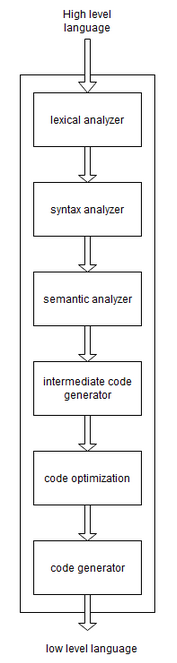
\includegraphics[width=30mm]{figure2.png}
   \end{center}
  \caption{Single Pass Compiler Process}
  \label{fig-sysdesov}
 \end{figure}

A multi pass compiler process, processes the source code through two phases: first pass  and second pass. The first pass includes a front end and analysis, performed by the lexical analyzer, syntax analyzer, semantic analyzer, resulting in the generation of intermediary code. The intermediary code is then passed on to the second pass. The second pass takes the IR code and performs the code optimization and code generation in the back end and synthesis, by converting the IR code appropriately to a desired low level language.[7] This means the analysis takes part in the front end pass one and the synthesis takes place in the back end of pass two. Resulting in the ability to separate the analysis of a high level code from the synthesis of the the low level code.

\pagebreak

\begin{figure}[hbt]
   \begin{center}
     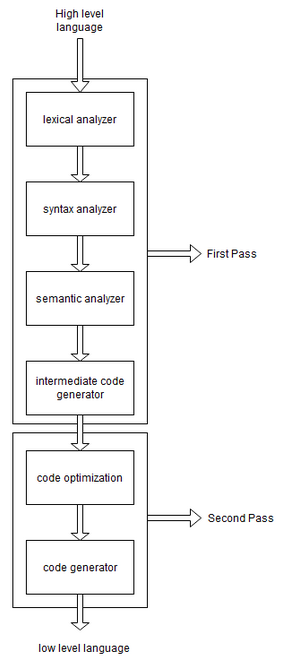
\includegraphics[width=60mm]{figure3.png}
   \end{center}
  \caption{Multi Pass Compiler Process}
  \label{fig-sysdesov}
 \end{figure}
 

Multi-pass compilers increase the portability of the compiler due to the separation of the front end in the first pass and the back end in the second pass. It makes it possible to customize the compiler for one high level language to many different machines. Likewise, it is possible to customize many different high level languages to a single machine. For these reasons, the AGC will be designed as a multi-pass compiler.


\subsection{Compiler vs. Interpreter}

Interpreters and Compilers translate source code written in higher-level languages, into a low-level machine readable language, using lexing and parsing before execution. The main difference between an interpreter and a compiler is that an interpreter directly executes instructions, while a compiler translates the source code to create an executable program [8]. Directly executing instructions is relatively slow but easy to debug since it will be obvious where an error occurs, but the compiler’s approach of compiling the source code before execution leads to faster execution times at the expense of more difficult debugging, and more memory needed for intermediary object code generation. In terms of this project, an interpreter for the AGP programming paradigm called Horde has been designed by Dr. Garcia and we will be working on designing a compiler for AGP code.


\section{Proposal}

The proposed compiler will use Flex for lexical analysis, Bison for semantic parsing, and  LLVM as an IR code to machine code translator to complete the AGC capable of rendering AGP code into assembly code for a given STM32 embedded system. 



\begin{figure}[hbt]
   \begin{center}
     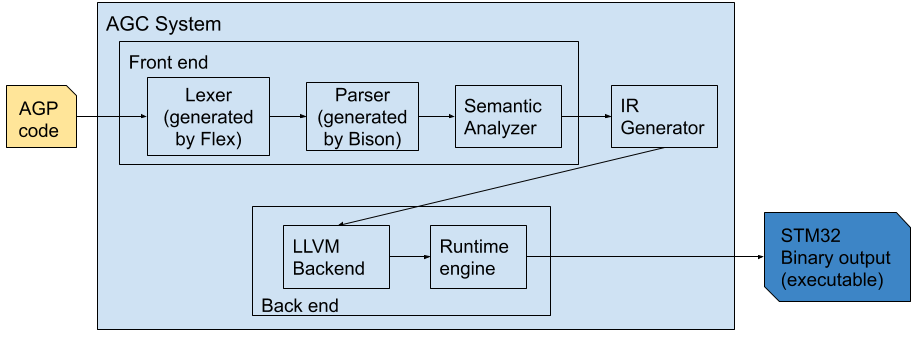
\includegraphics[width=170mm]{agcv2.png}
   \end{center}
  \caption{System design overview}
  \label{fig-sysdesov}
  \end{figure}



\subsection{Front End}

Initially, a lexer and parser are needed for analysis of the input code. We propose using Flex to generate a lexer to tokenize the input according to the rules defined by the regular expressions of AGP. We then propose using Bison to generate a parser to parse the tokens into a syntax tree. The parser analyzes the token arrangements in the tree to see if the syntax is correct (adhering to the source code grammar rules). Following the parser, semantic analysis is done  on the syntax tree: making sure identifiers and data types are compatible with each other, and that variables actually exist. The semantic analyzer produces an annotated syntax tree.

The annotated syntax tree (AST) is then used to generate intermediate representation (IR) code for the back end. We propose generating the IR as LLVM code.


\subsection{LLVM Translation}

LLVM is a compiler framework focused on a given front end, composed of: a parser for syntactic analysis of initial strings,  and a lexer which converts sequences of characters into tokens. The front end is then translated into an intermediate representation code (IR) by LLVM which is further optimized within. The back end is then a machine code representation of the IR which has been further translated to work on a desired target.

The LLVM Core libraries provide a modern source and target independent optimizer, along with code generation support for many popular CPUs. The libraries are built around a specified code representation known as the LLVM intermediate representation (LLVM IR).


\subsection{Runtime Engine}

An essential component of the runtime system is an abstract machine, which provides an intermediate language stage for computation [9].The runtime system has the purpose of implementing the language semantics of AGP by translating the abstract machine to physical. Some potential issues that can be expected when implementing parallel abstract machines such as for AGP are static and dynamic scheduling, granularity of tasks, distributed garbage collection, and code and thread migration [9].

\subsection{Testing}

The primary focus of the testing will be on the compilation functionality. Our tests will primarily focus on: validating the proper machine code generation, and assurance that machine code generated is according to the initial entry language specifications. In order to accomplish these primary objectives, a sizable set of small programs that demonstrate unique aspects of the AGP paradigm constitute a regression test suite. This regression test suite will then be the confirmation of the compiler creation progress if each iteration of the compiler passes the tests.
This testing method can be considered to fall under the black box method of testing due to the prioritization of system function and results, rather than a focus of optimization that would occur if we were to do white box testing.


\section{How the Project Relates to our Degrees}

A compiler is a complex software artifact. As we are all software engineering undergraduates, we have developed knowledge of current software theories and best practices. Compiler construction requires an understanding of programming languages, machine architecture, language theory, and algorithms. All of these concepts have been touched upon in numerous courses throughout the software engineering undergraduate degree, and this project will involve coordinating these skills to design and implement a compiler for the AGP paradigm. 

In SYSC 3120, we learned about requirements engineering. The background of this class regarding identifying and verifying requirement analysis will help clearly define the objectives of the project, and help mitigate risk. In SYSC 4120, we learned about system architecture, using the methodologies and structural models taught in this class when designing our system will help create a fluent detailed project model capable of modification. SYSC 3310 established first hand experience programming embedded systems in C. This directly translates into coding at the embedded level for our STM32 system. Furthermore, having taken numerous first and second year classes pertaining to C, we’ve established a foundational knowledge of C further solidifying a trust in the  main language we will be using in this project. In SYSC 4101, we studied different types of testing methods/practices. These will come into use once our system design is complete and implementation is in progress. It will allow us to follow the agile project development practice that is commonly used in the software development world.

	All these classes taken over the course of our university education play a role in the development, implementation, and testing of the AGC project.

\section{Skills we have to Complete Project}

Designing a compiler is a project based on software and computer knowledge. To undertake this project a solid understanding of requirements elicitation, software design, communication and research skills, software testing, and programming are required.  All team members are 4th year Software Engineering undergraduate students equipped with a suitable background for this project. Numerous courses have focused on the software design process, which have provided the skills needed to generate requirements, build models such as UML, use these models for implementation, and then to create well-built tests for verification of the system. All team members are familiar with version-control systems such as Git, and communication and research skills have been obtained and refined through courses such as CCDP 2100 and SYSC 3110, as well as through participation in many group projects. Majority of programming for this project will be done using C in the linux environment, which all team members have a strong understanding of from project and work experience.


\section{Methods to be Used}

In the design phase of the compiler, several choices have to be made about what software is best suited for our objective. 

One of the tools required for implementing the compiler is a lexer / scanner that converts the source text into tokens. Although possible to create our own from scratch, this would be infeasible given the timeline of the project. There are benefits of using aged and proven software that would generate and compile AGP much faster (and with fewer bugs) than we could ever create on our own. This leaves us to choose from available lexical analyzer generators, which will generate the lexers according to the regular expressions defined in AGP.

\begin{center}
\begin{tabular}{ |l | l|  }
 \hline
 \textbf{Lexer Generators} & \textbf{Notes} \\
 \hline 
 Flex & Generates parsers that are Look-Ahead Left to Right, or simply,\\ 
 	  &
 LALR, "a rewrite of lex intended to fix some of that tool's many bugs \\
 	  &
 and deficiencies." [10] \\ 
 \hline 
 Lex & predecessor to Flex, also LALR. \\
 \hline
\end{tabular}
\end{center}

\begin{center}
Table 1: Lexer generator options
\end{center}

Of the two, we choose to use Flex as it is newer, more readily available, has many bugs fixed from its predecessor, and is well suited to meet our objective. 

Another tool required for the compiler is a parser to take the tokens generated from the lexer and to output an abstract syntax tree (AST). Once again a parser could be created by hand, but there are plenty of parser generators such as BISON, YACC, and ANTLR.

\begin{center}
\begin{tabular}{ |l | l|  }
 \hline
 \textbf{Parser Generators} & \textbf{Notes} \\
 \hline 
 Bison & Newer version of Yacc, generates parsers that are LALR. No GUI,\\
       & but smaller memory requirements. \\
 \hline 
 Yacc & Older version of Bison, also LALR. \\
 \hline
 Antlr & Alternative, generates parser that are Left to Right, or  LL.\\
       & This may lead to issues with handling grammar. Generally \\
       & considered easier to use over Yacc/Bison. Uses more memory,\\
       & but has a GUI. \\
 \hline
\end{tabular}
\end{center}

\begin{center}
Table 2: Parser generator options
\end{center}

Of the three, we choose to use Bison, for many of the same reasons as we chose Flex. Bison is a newer and improved version of Yacc, and while it may be considered slightly harder to use over ANTLR, we feel that the memory advantage and Bison’s grammar handling will prove to be better suited for this project.

 LLVM will be used to construct, optimize and produce intermediate representation code which will then be translated into machine code. LLVM will act as a compiler framework, with a given front end composed of a parser and lexer from the Flex, Bison, and back end IR translator. Requirements Analysis will be used to define and analyze functional and nonfunctional requirements of the compiler system. With proper Requirements Analysis done prior to the project inception the compiler design and creation will be more seamless allowing for less re-work. 

Black box testing will be used to test the functionality of the program. Test suites will be created that assure that every function works as intended, and that the objectives are adequately met. The lexers/parsers shall be tested to ensure that they meet the requirements set by the language definitions of AGP. In addition, once the final iteration is complete, it shall be tested with moderately complex AGP code, as defined in the objective. These tests will decide whether the AGC project is a failure, a partial success, or a complete success.

\pagebreak

\section{Timetable with Milestones}

\begin{center}
\begin{tabular}{ |l | l | l|  }
 \hline
 \textbf{Task} & \textbf{Expected Completion Date} & \textbf{Notes} \\
 \hline 
 Research & September - October &  \\
 \hline 
 Design & Early November (Nov 7th)  & System architecture. \\
 \hline
 Prototype & Late November (Nov 28th) & Exploring LLVM, Flex, Bison, setting up development \\
 	    & & environments. \\
 \hline
 Testing & From Iteration 1 to Iteration 3 & Black box testing. \\
 \hline
 Progress Report & Jan 20th & Implementing a barebones compiler, likely\\
 		 & & with missing functionality, intended to test the design \\
 		 & & and method choices selected in the progress report.\\
 \hline
 Iteration 1 & Dec 12th  & Finish Iteration 1 before progress report, \\
 		 & & include results in report.\\
 \hline
 Iteration 2 & Jan 15th & Having learned what methods work from Iteration 1, \\
 		 & & the team will refine the design and implementation of \\ 		             		 & & the AGC system for better functionality, attempting \\
 		 & & to complete more compilation steps.\\
 \hline
 Iteration Final & Mar 15th & Improving on Iteration 2, at this point the design\\
 		 & & and implementation should be very familiar, with\\
 		 & & few/no bugs and a high degree of functionality in \\
 		 & & the system. Extensive documentation (diagrams, \\
 		 & & comments) will be done, as well as rigorous testing, \\
 		 & & to ensure a quality system.\\
 \hline
\end{tabular}
\end{center}

\begin{center}
Table 3: Task Scheduling
\end{center}

\pagebreak

\begin{figure}[hbt]
   \begin{center}
     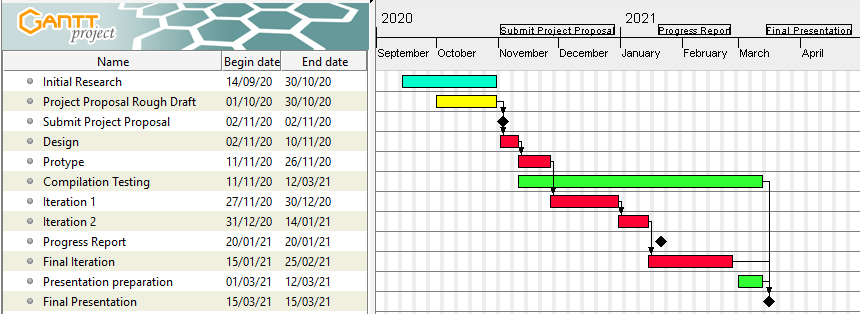
\includegraphics[width=170mm]{ganttchart.png}
   \end{center}
  \caption{Gantt Chart}
  \label{fig-sysdesov}
 \end{figure}

\subsection{Communication}

A private Discord server was created to facilitate written and verbal dialogs as well as share resources. Through Discord, recurring sprint meetings will be held Tuesdays and Fridays at 11 am EST. Github will be used for software version control to establish a project-wide repository.  Links to all relevant project resources will be in both the Github repository README and the Discord resources channel. All github prototype code will eventually evolve into the final code. Github also contains a kanban board to increase work/task progression and distribution transparency.

\section{Risks and Mitigation}

The lack of experience by all team members in compiler design is a risk to the successful implementation of the project. To remedy this, all members of the project have and continue to research extensively into compiler design using online documents, textbooks, reading papers, and articles. The members actively consult with the project supervisor for advice, guidance, and general help.
Our lack of experience in risks and mitigation is itself a risk. Having taken a requirements engineering class, we briefly touched on the topic of risks, however none of us have applied these skills on any projects. This final year project is a chance for us to out our learned skills acquired from requirements engineering.


\section{Components and Facilities Required}

The AGC must be compatible and function with a STM32 embedded test system, as specified by the project supervisor, Professor Garcia. The project will be made using the most current long term support version Ubuntu Linux 20.04 LTS. The majority of the code written will be in C. C is the primary supported language for the IR translator LLVM, C is a very fast and easy to use for middle level embedded programming. Clang will be used as the native LLVM C/C++/ Objective C compiler. Flex and Bison will be needed for the lexical analyzer and parser respectively, and as they are considered Unix utilities, are included in Ubuntu 20.04.



\section{Conclusion}

Through this project’s successful completion, we hope to expand the field of asynchronous graph programming by giving researchers a useful tool that can save time, increase efficiency, and allow for more branches of research. We deem this project a complete success when it can compile and execute any AGP code that we give it. We deem this project a partial success if the system can run moderately complex code, such as a program with several variable assignments, variable accesses, and recursive functions. 

\pagebreak

\begin{thebibliography}{9}

\bibitem{} 
N. Wirth, Compiler construction. Harlow: Addison-Wesley, 1996.

\bibitem{} 
J. Fryer and P. Garcia, "Towards a Programming Paradigm for Reconfigurable Computing: Asynchronous Graph Programming," 2020 25th IEEE International Conference on Emerging Technologies and Factory Automation (ETFA), Vienna, Austria, 2020, pp. 1721-1728, doi: 10.1109/ETFA46521.2020.9211968

\bibitem{}
B. Donyanavard, T. Muck, S. Sarma, and N. Dutt, “Sparta: Runtimetask allocation for energy efficient heterogeneous manycores,” in2016International Conference on Hardware/Software Codesign and SystemSynthesis (CODES  ISSS). IEEE, 2016, pp. 1–10.

\bibitem{}
M. A. Aguilar, R. Leupers, G. Ascheid, and L. G. Murillo, “Automaticparallelization and accelerator offloading for embedded applications on heterogeneous mpsocs,” in Proceedings of the 53rd Annual DesignAutomation Conference. ACM, 2016, p. 49

\bibitem{} 
S. Marlow, "Fighting spam with Haskell - Facebook Engineering", Facebook Engineering, 2020. [Online]. Available: \url{https://engineering.fb.com/2015/06/26/security/fighting-spam-with-haskell/} 
[Accessed: 26- Oct- 2020]

\bibitem{}
T. Avacheva and A. Prutzkow, “The Evolution of Imperative Programming Paradigms as a Search for New Ways to Reduce Code Duplication,” IOP Conference Series: Materials Science and Engineering, vol. 714, p. 012001, 2020.

\bibitem{}
W. M. Waite, G. Goos, “Compiler Construction”, Karlsruhe 22nd February 1996, [Online] Available: https://www.cs.cmu.edu/~aplatzer/course/Compilers/waitegoos.pdf, p. 1-9

\bibitem{}
A. V. Aho, M. S. Lam, R. Sethi, and J. D. Ullman, Compilers: principles, techniques, and tools. India: Pearson India Education Services, 2015, p. 2-3

\bibitem{}
S. Diehl, P. Hartel, and P. Sestoft, “ Abstract machines for programming language implementation” Future Generation Computer Systems 2000


\bibitem{}
Levine, J. R. (2009). Preface. In 1024727333 786678555 S. S. Laurent (Ed.), Flex \& Bison (1st ed., p. 17). O'Reily.



\end{thebibliography}

\end{document}
